\chapter{Couleur et absorbance}\label{ch:g11:absorbance}

Sur le banc d'une salle de sport, une bouteille de boisson énergétique
brille d'un bleu vif. Sa couleur vient d'un colorant qui y est dissous,
à raison de quelques milligrammes pour un litre entier~: bien trop peu
pour être pesé, et bien trop peu pour être vu à l'état solide. Un
laboratoire d'analyse alimentaire doit pourtant contrôler cette
quantité, car un colorant ne peut être ajouté que dans certaines
limites. La couleur elle-même est la clé. Plus une solution contient de
colorant, plus elle absorbe de lumière~; un instrument qui mesure la
lumière absorbée par une solution mesure, en fait, une concentration.

\begin{recall}
Les \omterm{def:g10:concentration-and-dilution:mass-concentration}{concentrations massique} et molaire d'une solution~; la \omterm{def:g10:concentration-and-dilution:dilution}{dilution}
d'une \omterm{def:g10:concentration-and-dilution:dilution}{solution mère}~; une \omterm{def:g10:concentration-and-dilution:standard}{échelle de teintes} de \omterm{def:g10:concentration-and-dilution:standard}{solutions étalons}
comparée à une solution inconnue (\cref{ch:g10:concentration-and-dilution}).
\end{recall}

\begin{omfigure}
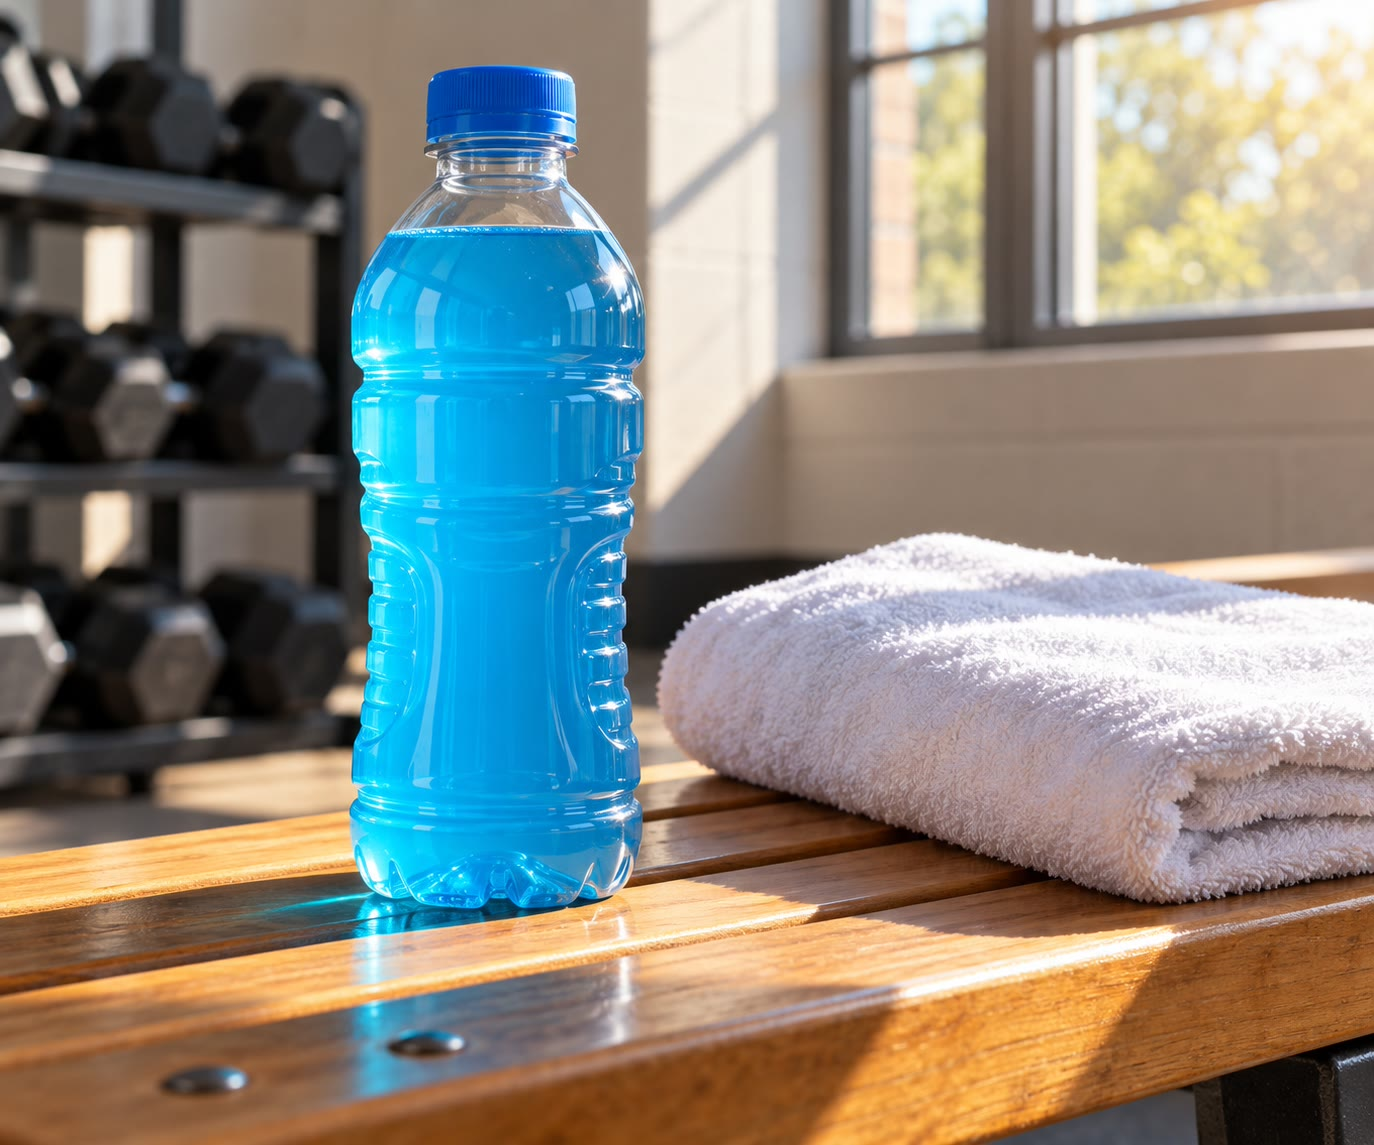
\includegraphics[width=0.5\linewidth]{images/book1/ai/g11-sports-drink.jpg}

{\small Une boisson bleue~: sa couleur vient de quelques milligrammes de
colorant par litre.}
\end{omfigure}

\section{La couleur d'une solution}

La lumière blanche, comme celle du jour, est un \omterm{def:g6:pure-substances-and-mixtures:mixture}{mélange} de toutes les
couleurs de l'arc-en-ciel. À chaque couleur correspond une longueur
d'onde, d'environ \qty{400}{nm} pour le violet à environ \qty{750}{nm}
pour le rouge~; le livre de physique explique ce qu'est une longueur
d'onde, et elle ne sert ici que d'étiquette pour une couleur. Une
solution colorée absorbe une partie de la lumière qui la traverse,
certaines couleurs beaucoup plus que d'autres~; l'œil voit les couleurs
qui passent.

\begin{definition}[Couleurs complémentaires]\label{def:g11:absorbance:complementary}
Deux couleurs sont des \emph{couleurs complémentaires}\index{couleurs complementaires@couleurs complémentaires}
si leur \omterm{def:g6:pure-substances-and-mixtures:mixture}{mélange} donne de la lumière blanche. Sur un cercle chromatique,
deux couleurs complémentaires sont diamétralement opposées.
\end{definition}

\begin{omfigure}
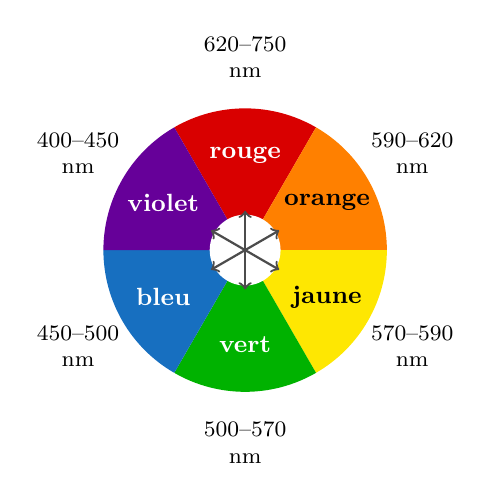
\begin{tikzpicture}[font=\small]
  \foreach \a/\c/\n/\w/\t in {90/red!85!black/rouge/{620--750}/white,
      30/orange/orange/{590--620}/black, -30/yellow!90!orange/jaune/{570--590}/black,
      -90/green!70!black/vert/{500--570}/white, -150/cyan!50!blue/bleu/{450--500}/white,
      150/violet!80!blue/violet/{400--450}/white} {
    \fill[\c] (0,0) -- (\a-30:1.8) arc[start angle=\a-30, end angle=\a+30,
      radius=1.8] -- cycle;
    \node[text=\t, font=\small\bfseries] at (\a:1.2) {\n};
    \node[font=\footnotesize, align=center] at (\a:2.45) {\w\\ nm};
  }
  \fill[white] (0,0) circle (0.45);
  \draw[<->, thick, black!70] (90:0.5) -- (-90:0.5);
  \draw[<->, thick, black!70] (30:0.5) -- (-150:0.5);
  \draw[<->, thick, black!70] (-30:0.5) -- (150:0.5);
\end{tikzpicture}

{\small Un cercle chromatique, avec des longueurs d'onde approximatives.
Les \omterm{def:g11:absorbance:complementary}{couleurs complémentaires} sont face à face~: le rouge et le vert,
l'orange et le bleu, le jaune et le violet.}
\end{omfigure}

\begin{proposition}[La couleur perçue]\label{prop:g11:absorbance:colour-seen}
Une solution qui absorbe principalement une couleur de la lumière
blanche prend la couleur complémentaire de celle-ci.
\end{proposition}

\begin{proof}
Admis~: la lumière qui passe est la lumière blanche privée de la couleur
absorbée, et l'œil perçoit ce reste comme la couleur complémentaire.
\end{proof}

\begin{example}[Deux colorants alimentaires]\label{ex:g11:absorbance:dyes}
% ledger: lmax:E133, lmax:E102
Le colorant bleu de la boisson, appelé bleu brillant (E133), absorbe
surtout la lumière rouge-orangé, vers \qty{629}{nm}~: il paraît bleu. Le
colorant jaune tartrazine (E102) absorbe surtout la lumière bleu-violet,
vers \qty{427}{nm}~: il paraît jaune. Une boisson verte contient en
général les deux.
\end{example}

\section{Le spectre d'absorption}

\begin{definition}[Spectre d'absorption]\label{def:g11:absorbance:spectrum}
Le \emph{spectre d'absorption}\index{spectre d'absorption} d'une
solution est le graphique de la lumière qu'elle absorbe (son \omterm{def:g11:absorbance:absorbance}{absorbance},
définie à la section suivante) en fonction de la longueur d'onde. La
longueur d'onde pour laquelle l'absorption est la plus forte se note
$\lambda_{\max}$.
\end{definition}

\begin{omfigure}
\begin{tikzpicture}
\begin{axis}[width=0.85\linewidth, height=6cm, xmin=380, xmax=750,
    ymin=0, ymax=0.95, xlabel={longueur d'onde $\lambda$ (\si{nm})},
    ylabel={absorbance $A$}, axis lines*=left, ymajorgrids,
    grid style={gray!20}, tick label style={font=\small},
    label style={font=\small}, xtick={400,450,500,550,600,650,700,750},
    ]
  % ledger: lmax:E133, abs:E133, lmax:E102, abs:E102 (band shapes synthetic)
  \addplot[very thick, cyan!60!blue] table[x=lambda, y=E133]
    {figdata/out/grade-11-absorbance-a.dat};
  \addplot[very thick, orange!85!yellow] table[x=lambda, y=E102]
    {figdata/out/grade-11-absorbance-a.dat};
  \node[font=\small, align=left, anchor=west, text=cyan!60!blue!80!black]
    at (axis cs:668,0.62) {colorant bleu E133,\\ \qty{5.0}{mg/L}};
  \node[font=\small, align=left, anchor=west, text=orange!80!black]
    at (axis cs:470,0.66) {colorant jaune E102,\\ \qty{15}{mg/L}};
  \addplot[dashed, black!50] coordinates {(629,0) (629,0.82)};
  \addplot[dashed, black!50] coordinates {(427,0) (427,0.795)};
  \node[font=\small, anchor=south] at (axis cs:629,0.83) {\qty{629}{nm}};
  \node[font=\small, anchor=south] at (axis cs:427,0.81) {\qty{427}{nm}};
\end{axis}
\end{tikzpicture}

{\small \omterm{def:g11:absorbance:spectrum}{Spectres d'absorption} des deux colorants dans l'eau, dans une
cuve de \qty{1}{cm} d'épaisseur. La forme des bandes est tracée à partir
d'un modèle simple~; la position des maximums et leur hauteur sont
celles des spécifications des deux colorants.}
\end{omfigure}

\begin{remark}[Lire un spectre]\label{rem:g11:absorbance:reading}
Le colorant bleu n'absorbe presque rien au-dessous de \qty{520}{nm}~: la
lumière bleue et violette passe, et la solution paraît bleue. Le
colorant jaune n'absorbe presque rien au-dessus de \qty{520}{nm}~: la
lumière verte, jaune, orange et rouge passe, et l'œil voit du jaune. À
\qty{629}{nm}, seul le colorant bleu absorbe~; à \qty{427}{nm}, presque
seulement le jaune.
\end{remark}

\section{L'absorbance et le spectrophotomètre}

\begin{definition}[Absorbance]\label{def:g11:absorbance:absorbance}
L'\emph{absorbance}\index{absorbance} $A$ d'une solution, à une longueur
d'onde choisie, est le nombre affiché par un spectrophotomètre qui
mesure la part de la lumière de cette longueur d'onde absorbée par la
solution. Elle n'a pas d'unité~; elle est nulle pour le \omterm{def:g6:solutions-and-solubility:solute}{solvant} pur, et
d'autant plus grande que la solution absorbe de lumière.
\end{definition}

\begin{omfigure}
\begin{tikzpicture}[font=\small]
  % lamp
  \shade[ball color=yellow!40] (0,0.6) circle (0.32);
  \foreach \a in {0,45,90,135,180,225,270,315} \draw[yellow!60!orange, thick] (\a:0.4) ++(0,0.6) -- ++(\a:0.18);
  \node[anchor=north] at (0,-0.25) {lampe};
  \draw[black!60, thick] (0.8,0.6) -- (1.75,0.6);
  % prism
  \fill[cyan!10, draw=black!60] (1.75,0.15) -- (2.55,0.15) -- (2.15,1.15) -- cycle;
  \node[anchor=north] at (2.15,-0.25) {prisme};
  \foreach \c/\d in {violet/0.35, blue/0.22, green!70!black/0.08, yellow!90!orange/-0.06,
      orange/-0.2, red/-0.34}
    \draw[\c, thick] (2.45,0.6) -- (3.45,{0.6+\d});
  % slit
  \fill[black!70] (3.5,0.92) rectangle (3.6,1.4);
  \fill[black!70] (3.5,-0.2) rectangle (3.6,0.52);
  \node[anchor=north] at (3.55,-0.25) {fente};
  \draw[orange, very thick] (3.6,0.6) -- (4.75,0.6);
  % cuvette
  \pic (cv) at (5,0) {cuvette={0.75}{cyan!50!blue!45}};
  \node[anchor=north] at (5,-0.25) {cuve};
  \draw[orange!60, thick] (5.3,0.6) -- (6.3,0.6);
  % detector and display
  \fill[black!15, draw=black!60] (6.3,0.2) rectangle (6.9,1.0);
  \node[anchor=north] at (6.6,-0.25) {détecteur};
  \draw[black!60] (6.9,0.6) -- (7.4,0.6);
  \fill[black!80, draw=black] (7.4,0.25) rectangle (9.4,0.95);
  \node[green!70!white, font=\footnotesize\ttfamily] at (8.4,0.6) {A = 0.590};
  \node[anchor=north] at (8.4,-0.25) {affichage};
\end{tikzpicture}

{\small Principe d'un spectrophotomètre. Un prisme décompose la lumière
blanche en ses couleurs~; une fente ne laisse passer qu'une longueur
d'onde, choisie par l'utilisateur~; le détecteur compare la lumière qui
sort de la cuve à celle qui y entre, et l'écran affiche l'\omterm{def:g11:absorbance:absorbance}{absorbance}.}
\end{omfigure}

\begin{remark}[D'où vient ce nombre]\label{rem:g11:absorbance:log}
L'instrument calcule l'\omterm{def:g11:absorbance:absorbance}{absorbance} à partir des intensités de la lumière
qui entre dans la solution et qui en sort, à l'aide d'une fonction
mathématique rencontrée en dernière année de lycée, le logarithme. Un
volume universitaire donne la formule~; ici, l'\omterm{def:g11:absorbance:absorbance}{absorbance} est simplement
ce que lit l'instrument.
\end{remark}

\begin{inthelab}[Faire le zéro du spectrophotomètre]
La cuve, le \omterm{def:g6:solutions-and-solubility:solute}{solvant} et l'instrument lui-même absorbent un peu de
lumière. Avant toute mesure, on place dans l'instrument une cuve remplie
du \omterm{def:g6:solutions-and-solubility:solute}{solvant} pur, le \emph{blanc}, et on règle l'appareil pour qu'il
indique $A = 0$ à la longueur d'onde choisie. Chaque mesure qui suit est
l'\omterm{def:g11:absorbance:absorbance}{absorbance} du \omterm{def:g6:solutions-and-solubility:solute}{soluté} seul. On tient toujours les cuves par leurs faces
dépolies, et on les essuie~: une trace de doigt sur une face
transparente absorbe aussi de la lumière.
\end{inthelab}

\begin{omfigure}
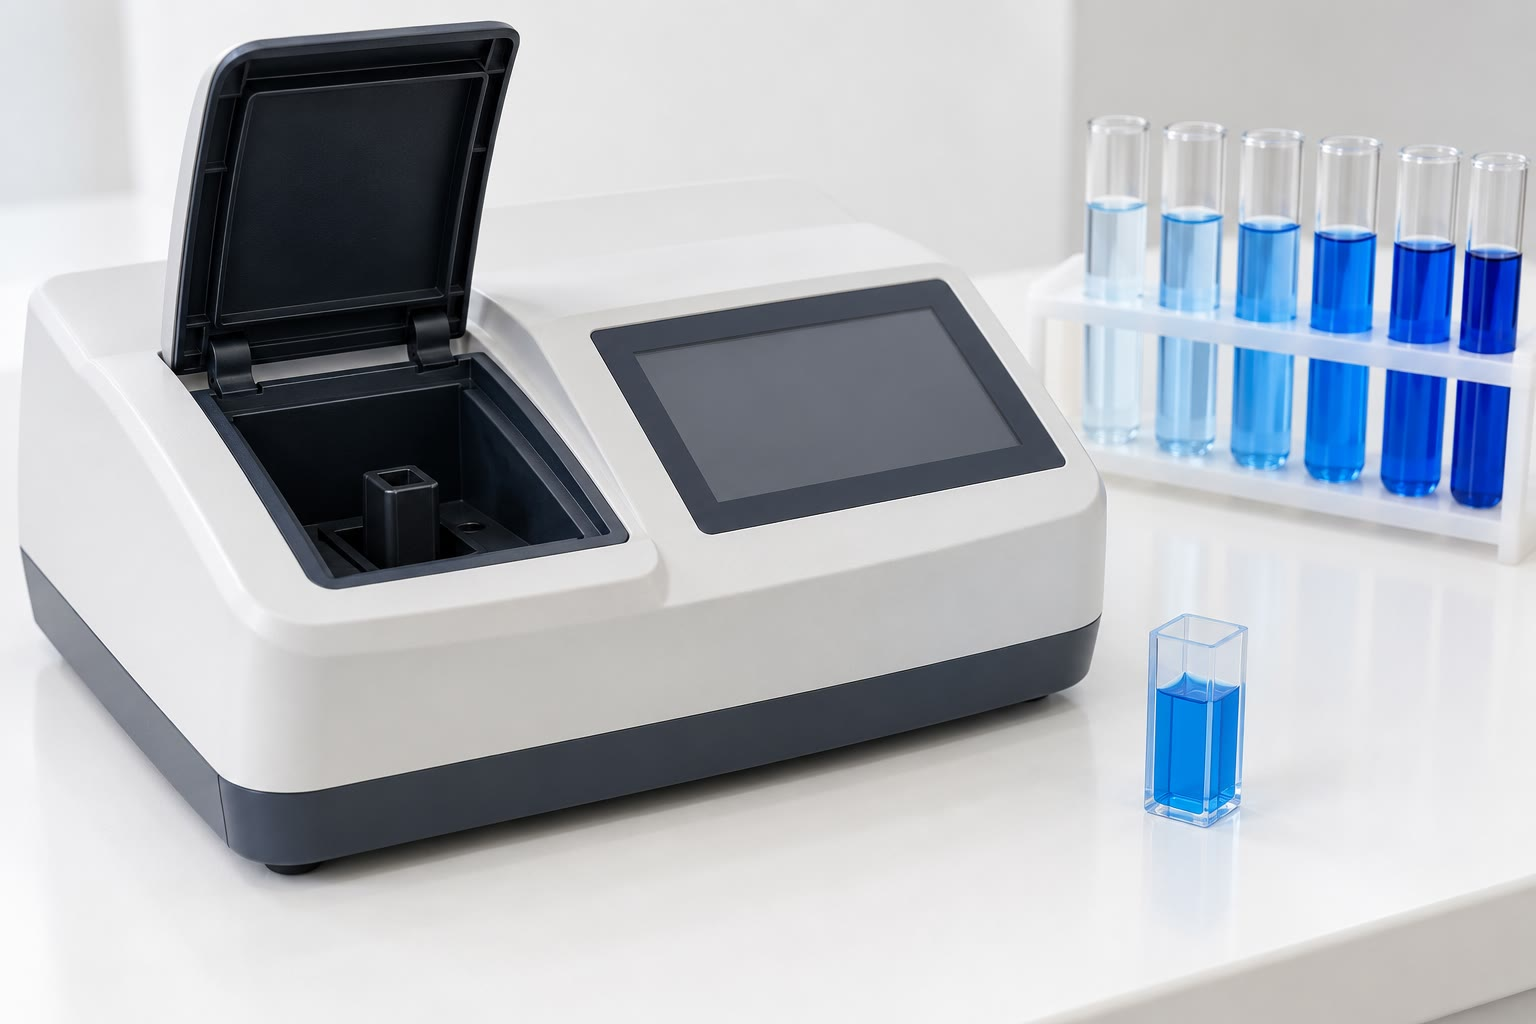
\includegraphics[width=0.5\linewidth]{images/book1/ai/g11-spectrophotometer.jpg}

{\small Un spectrophotomètre et ses cuves carrées.}
\end{omfigure}

\section{La loi de Beer--Lambert}

\begin{definition}[Coefficient d'absorption molaire]\label{def:g11:absorbance:epsilon}
Le \emph{coefficient d'absorption molaire}\index{coefficient d'absorption molaire}
$\varepsilon$ d'une espèce dissoute, à une longueur d'onde donnée,
mesure avec quelle force une \omterm{def:g10:the-mole:amount}{mole} de cette espèce absorbe la lumière~;
il dépend de l'espèce, du \omterm{def:g6:solutions-and-solubility:solute}{solvant} et de la longueur d'onde, et
s'exprime en \si{L/(mol.cm)}.
\end{definition}

\begin{proposition}[Loi de Beer--Lambert]\label{prop:g11:absorbance:beer-lambert}
Pour une solution diluée d'une seule espèce absorbante, de \omterm{def:g10:concentration-and-dilution:molar-concentration}{concentration
molaire} $c$, dans une cuve d'épaisseur $\ell$, l'\omterm{def:g11:absorbance:absorbance}{absorbance} à une
longueur d'onde donnée vaut
\[
  A = \varepsilon\, \ell\, c .
\]
L'\omterm{def:g11:absorbance:absorbance}{absorbance} est proportionnelle à la concentration.
\end{proposition}

\begin{proof}
Admis ici~; la démonstration figure dans un volume universitaire.
\end{proof}


\begin{remark}[Avec une concentration massique]\label{rem:g11:absorbance:mass}
% ledger: abs:E133, mw:E133
Comme $c = C_m / M$, la loi s'écrit aussi $A = a\, \ell\, C_m$, avec
$a = \varepsilon / M$ en \si{L/(g.cm)}. Les spécifications des colorants
alimentaires donnent $a$~: pour le colorant bleu E133 à \qty{629}{nm}, $a =
\qty{164}{L/(g.cm)}$, et avec sa \omterm{def:g10:the-mole:molar-mass}{masse molaire} de \qty{792.9}{g/mol},
$\varepsilon = 164 \times 792.9 = \qty{1.30e5}{L/(mol.cm)}$. Une solution
qui n'en contient que \qty{5.0}{mg/L}, dans une cuve de \qty{1}{cm},
donne déjà
$A = 164 \times 1 \times 0.0050 = 0.82$.
\end{remark}

\begin{remark}[Solutions diluées seulement]\label{rem:g11:absorbance:dilute}
La proportionnalité n'est valable que pour les solutions diluées, en
pratique pour des \omterm{def:g11:absorbance:absorbance}{absorbances} inférieures à 1 ou 1.5 environ sur un
appareil ordinaire. Une solution trop concentrée est diluée d'un facteur
connu avant d'être mesurée.
\end{remark}

\section{Mesurer une concentration}

\begin{definition}[Droite d'étalonnage]\label{def:g11:absorbance:calibration-line}
Une \emph{droite d'étalonnage}\index{droite d'etalonnage@droite d'étalonnage} est le
graphique de l'\omterm{def:g11:absorbance:absorbance}{absorbance} d'une série de \omterm{def:g10:concentration-and-dilution:standard}{solutions étalons} d'une même
espèce, mesurée à la même longueur d'onde dans la même cuve, en fonction
de leur concentration. Quand la loi de Beer--Lambert est vérifiée, c'est
une droite passant par l'origine.
\end{definition}

\begin{method}[Mesurer une concentration à l'aide d'une droite d'étalonnage]\label{met:g11:absorbance:calibration}
\begin{enumerate}
  \item Enregistrer le \omterm{def:g11:absorbance:spectrum}{spectre d'absorption} de l'espèce et choisir la
        longueur d'onde $\lambda_{\max}$, où l'\omterm{def:g11:absorbance:absorbance}{absorbance} est la plus
        grande et varie le moins pour une petite erreur sur la longueur
        d'onde.
  \item Faire le zéro de l'instrument avec le blanc.
  \item Préparer des \omterm{def:g10:concentration-and-dilution:standard}{solutions étalons} par \omterm{def:g10:concentration-and-dilution:dilution}{dilution} d'une \omterm{def:g10:concentration-and-dilution:dilution}{solution mère}
        et mesurer leurs \omterm{def:g11:absorbance:absorbance}{absorbances}.
  \item Tracer $A$ en fonction de la concentration et tracer la droite
        passant par l'origine la plus proche des points.
  \item Mesurer l'inconnue, diluée si nécessaire pour que son \omterm{def:g11:absorbance:absorbance}{absorbance}
        se situe parmi celles des étalons, et lire sa concentration sur
        la droite (ou diviser $A$ par le coefficient directeur)~;
        multiplier par le \omterm{def:g10:concentration-and-dilution:dilution}{facteur de dilution}.
\end{enumerate}
\end{method}

\begin{omfigure}
\begin{tikzpicture}
\begin{axis}[width=0.72\linewidth, height=6cm, xmin=0, xmax=5.6,
    ymin=0, ymax=0.95, xlabel={concentration en E133 (\si{mg/L})},
    ylabel={absorbance à \qty{629}{nm}}, axis lines*=left, ymajorgrids,
    xmajorgrids, grid style={gray!20}, tick label style={font=\small},
    label style={font=\small}]
  % ledger: abs:E133 (points synthetic: exact values + fixed offsets)
  \addplot[only marks, mark=*, mark size=2.2pt, omDef] table[x=C, y=A]
    {figdata/out/grade-11-absorbance-b.dat};
  \addplot[thick, omProp, domain=0:5.5] {0.164*x};
  \addplot[dashed, black!60] coordinates {(0,0.590) (3.6,0.590) (3.6,0)};
  \node[font=\small, anchor=south west] at (axis cs:0.1,0.6) {inconnue~: $A = 0.590$};
  \node[font=\small, anchor=west] at (axis cs:3.65,0.22) {\qty{3.6}{mg/L}};
\end{axis}
\end{tikzpicture}

{\small \omterm{def:g11:absorbance:calibration-line}{Droite d'étalonnage} du colorant bleu~: cinq étalons (les points)
et la droite passant par l'origine, de coefficient directeur
\qty{0.164}{L/mg}. Une inconnue qui donne $A = 0.590$ a une
concentration de $0.590 / 0.164 =
\qty{3.6}{mg/L}$.}
\end{omfigure}

\begin{example}[Les cinq étalons]\label{ex:g11:absorbance:standards}
On dilue une \omterm{def:g10:concentration-and-dilution:dilution}{solution mère} du colorant bleu à \qty{100}{mg/L} pour
obtenir \qty{100.0}{mL} de chaque étalon~: pour \qty{2.0}{mg/L}, le
\omterm{def:g10:concentration-and-dilution:dilution}{facteur de dilution} vaut 50, donc on complète \qty{2.0}{mL} de \omterm{def:g10:concentration-and-dilution:dilution}{solution
mère} à \qty{100.0}{mL}. Les cinq étalons, de 1 à \qty{5}{mg/L}, donnent
0.168, 0.325, 0.494, 0.652 et 0.823~: à quelques millièmes près
$0.164 \times C$, la droite de la figure.
\end{example}

\section{Exercices}

\begin{exercise}[$\star$]\label{exo:g11:absorbance:1}
Une solution absorbe principalement la lumière orange. De quelle couleur
paraît-elle~? Et une solution qui absorbe principalement la lumière
violette~?
\end{exercise}

\begin{exercise}[$\star$]\label{exo:g11:absorbance:2}
À l'aide du cercle chromatique, donner la couleur principalement
absorbée par une solution verte, et le domaine de longueurs d'onde
qu'occupe cette couleur.
\end{exercise}

\begin{exercise}[$\star$]\label{exo:g11:absorbance:3}
Lire sur les \omterm{def:g11:absorbance:spectrum}{spectres d'absorption} la longueur d'onde $\lambda_{\max}$
de chaque colorant et son \omterm{def:g11:absorbance:absorbance}{absorbance} à cette longueur d'onde.
\end{exercise}

\begin{exercise}[$\star$]\label{exo:g11:absorbance:4}
Une solution de colorant à \qty{2.0}{mg/L} donne $A = 0.30$. Quelle
\omterm{def:g11:absorbance:absorbance}{absorbance} donne une solution du même colorant à \qty{6.0}{mg/L}, dans la
même cuve, à la même longueur d'onde~? Et à \qty{1.0}{mg/L}~?
\end{exercise}

\begin{exercise}[$\star$]\label{exo:g11:absorbance:5}
Qu'est-ce que le blanc d'un spectrophotomètre, et pourquoi fait-on le
zéro de l'instrument avec lui~?
\end{exercise}

\begin{exercise}[$\star\star$]\label{exo:g11:absorbance:6}
À l'aide de la \omterm{def:g11:absorbance:calibration-line}{droite d'étalonnage} du colorant bleu, trouver la
concentration d'une solution qui donne $A = 0.41$.
\end{exercise}

\begin{exercise}[$\star\star$]\label{exo:g11:absorbance:7}
Pour doser le colorant bleu, pourquoi régler le spectrophotomètre sur
\qty{629}{nm} plutôt que sur \qty{550}{nm}~? Donner deux raisons.
\end{exercise}

\begin{exercise}[$\star\star$]\label{exo:g11:absorbance:8}
Une boisson non diluée donne $A = 2.4$ à \qty{629}{nm}, une valeur trop
élevée pour être fiable. On la dilue cinq fois, et elle donne alors
$A = 0.48$. Trouver la concentration de colorant bleu dans la boisson.
\end{exercise}

\begin{exercise}[$\star\star$]\label{exo:g11:absorbance:9}
% ledger: mw:E102, abs:E102
Une solution de tartrazine à \qty{15.0}{mg/L} donne $A = 0.795$ à
\qty{427}{nm} dans une cuve de \qty{1.00}{cm}. Calculer son coefficient
d'absorption massique $a$ en \si{L/(g.cm)}, puis son \omterm{def:g11:absorbance:epsilon}{coefficient
d'absorption molaire} (\omterm{def:g10:the-mole:molar-mass}{masse molaire} \qty{534.4}{g/mol}).
\end{exercise}

\begin{exercise}[$\star\star$]\label{exo:g11:absorbance:10}
Observer les spectres des deux colorants. Au-dessus de quelle longueur
d'onde le colorant jaune n'absorbe-t-il presque plus~? Pourquoi
peut-on doser le colorant bleu à \qty{629}{nm} même dans une boisson
verte qui contient aussi le colorant jaune~?
\end{exercise}

\begin{exercise}[$\star\star$]\label{exo:g11:absorbance:11}
On mesure la même solution dans une cuve de \qty{2.0}{cm} d'épaisseur au
lieu de \qty{1.0}{cm}. Comment son \omterm{def:g11:absorbance:absorbance}{absorbance} change-t-elle~? Pourquoi~?
\end{exercise}

\begin{exercise}[$\star\star\star$]\label{exo:g11:absorbance:12}
Des étalons du colorant bleu à 5, 10, 20 et \qty{40}{mg/L} donnent 0.82,
1.62, 2.30 et 2.70. Calculer $A / C$ pour chacun. Que remarque-t-on~?
Quels étalons peut-on utiliser pour une \omterm{def:g11:absorbance:calibration-line}{droite d'étalonnage}, et que
faut-il faire d'une inconnue qui donne $2.5$~?
\end{exercise}

\begin{exercise}[$\star\star\star$]\label{exo:g11:absorbance:13}
Une boisson verte contient le colorant bleu et le colorant jaune. Dans
une cuve de \qty{1.00}{cm}, elle donne $A = 0.574$ à \qty{629}{nm} et
$A = 0.53$ à \qty{427}{nm}. À \qty{427}{nm}, le colorant bleu n'absorbe
presque rien, et à \qty{629}{nm} le colorant jaune n'absorbe rien.
Trouver les \omterm{def:g10:concentration-and-dilution:mass-concentration}{concentrations massiques} des deux colorants (utiliser
$a = \qty{164}{L/(g.cm)}$ et
$a = \qty{53.0}{L/(g.cm)}$).
\end{exercise}

\begin{exercise}[$\star\star\star$]\label{exo:g11:absorbance:14}
Une élève oublie le blanc et fait le zéro de l'instrument avec une cuve
vide. Chaque mesure est alors trop élevée de \num{0.040}. L'inconnue
donne $0.368$, et elle divise par le coefficient directeur $0.164$ de la
vraie \omterm{def:g11:absorbance:calibration-line}{droite d'étalonnage}. Quelle concentration trouve-t-elle~? Quelle
est la vraie~? De quel pourcentage se trompe-t-elle~?
\end{exercise}

\begin{exercise}[$\star\star\star$]\label{exo:g11:absorbance:15}
% ledger: adi:E102
La dose journalière admissible de tartrazine est de \qty{10}{mg} par
kilogramme de masse corporelle. Une boisson en contient \qty{20}{mg/L}.
Quel volume de boisson amènerait un adulte de \qty{60}{kg} à cette dose
en une journée~? Ce risque est-il réaliste~?
\end{exercise}

\section{Problème~: le bleu d'une boisson énergétique}


\begin{problem}[{Problème du week-end --- combien de bouteilles d'une
boisson énergétique bleue un enfant devrait-il boire pour atteindre la
limite journalière sans risque de son colorant~?}]
\label{pb:g11:absorbance:1}
% ledger: lmax:E133, abs:E133, mw:E133, adi:E133
Un laboratoire d'analyse alimentaire contrôle le colorant bleu E133
d'une boisson énergétique vendue en bouteilles de \qty{500}{mL}. Les
spécifications du colorant donnent sa \omterm{def:g10:the-mole:molar-mass}{masse molaire}, \qty{792.9}{g/mol},
et sa dose journalière admissible~: \qty{6}{mg} par kilogramme de masse
corporelle et par jour, une quantité qui peut être consommée chaque jour
pendant toute une vie sans risque appréciable.

\medskip
\noindent\textbf{Partie I --- Couleur et spectre.}
\begin{enumerate}
  \item La boisson paraît bleue. À l'aide du cercle chromatique,
        déterminer la couleur de lumière qu'elle absorbe le plus.
  \item Lire la longueur d'onde $\lambda_{\max}$ du colorant sur son
        spectre.
  \item Pourquoi l'\omterm{def:g11:absorbance:absorbance}{absorbance} du colorant est-elle presque nulle à
        \qty{450}{nm}~? Est-ce cohérent avec sa couleur~?
  \item À quelle longueur d'onde faut-il faire les mesures~?
\end{enumerate}

\medskip
\noindent\textbf{Partie II --- La \omterm{def:g11:absorbance:calibration-line}{droite d'étalonnage}.}
\begin{enumerate}[resume]
  \item On dissout \qty{50.0}{mg} de colorant pur pour obtenir
        \qty{500.0}{mL} de \omterm{def:g10:concentration-and-dilution:dilution}{solution mère}. Calculer sa \omterm{def:g10:concentration-and-dilution:mass-concentration}{concentration
        massique} en \si{mg/L}.
  \item On prépare des étalons à 1.0, 2.0, 3.0, 4.0 et \qty{5.0}{mg/L},
        \qty{100.0}{mL} chacun. Quel volume de \omterm{def:g10:concentration-and-dilution:dilution}{solution mère} faut-il pour
        l'étalon à \qty{3.0}{mg/L}~? Avec quelle verrerie~?
  \item Les étalons donnent 0.168, 0.325, 0.494, 0.652 et 0.823. Calculer
        $A / C$ pour chacun, et montrer que les points sont proches d'une
        droite passant par l'origine, de coefficient directeur voisin de
        \qty{0.164}{L/mg}.
  \item Pourquoi la droite doit-elle passer par l'origine~?
  \item En déduire le coefficient d'absorption massique $a$ du colorant
        en \si{L/(g.cm)} (cuve de \qty{1.00}{cm}), puis son \omterm{def:g11:absorbance:epsilon}{coefficient
        d'absorption molaire}.
\end{enumerate}

\medskip
\noindent\textbf{Partie III --- La boisson.}
\begin{enumerate}[resume]
  \item On complète \qty{25.0}{mL} de boisson à \qty{50.0}{mL} avec de
        l'eau. Quel est le \omterm{def:g10:concentration-and-dilution:dilution}{facteur de dilution}~?
  \item La boisson diluée donne $A = 0.590$. Trouver sa concentration en
        colorant.
  \item En déduire la concentration en colorant de la boisson elle-même.
  \item Quelle \omterm{def:g11:absorbance:absorbance}{absorbance} donnerait la boisson non diluée~? Pourquoi
        l'a-t-on diluée~?
  \item Calculer la masse de colorant d'une bouteille.
  \item Calculer la quantité de colorant, en \omterm{def:g10:the-mole:amount}{moles}, d'une bouteille.
\end{enumerate}

\medskip
\noindent\textbf{Partie IV --- La dose journalière admissible.}
\begin{enumerate}[resume]
  \item Quelle masse de colorant un enfant de \qty{30}{kg} peut-il
        absorber chaque jour~?
  \item Combien de bouteilles l'enfant devrait-il boire en une journée
        pour l'atteindre~?
  \item Quel volume de boisson cela représente-t-il~? Commenter.
  \item Même question pour un adulte de \qty{70}{kg}.
  \item Donner la réponse finale~: combien de bouteilles de
        \qty{500}{mL} un enfant de \qty{30}{kg} devrait-il boire en une
        journée pour atteindre la dose journalière admissible du
        colorant~?
\end{enumerate}
\end{problem}
